%===========================================================
%不尽完善之处尽情谅解!
%如果需要帮助可以发邮件到zpc126@163.com!
%===========================================================
\documentclass{ctexart}
\usepackage{paracol}
\usepackage{hyperref}
\usepackage{lipsum}
\usepackage{transparent}
\usepackage{graphicx}
\usepackage{graphics}
\usepackage{tcolorbox}
\usepackage{fontawesome}
\usepackage{array}
\usepackage[top=0.5cm,right=0.5cm,left=0.5cm,bottom=0.5cm,a4paper]{geometry}
%-------------------------------------
%          定义背景颜色
%-------------------------------------
\usepackage{xcolor}
\definecolor{headcol}{gray}{0.5}
\definecolor{rbgcol}{RGB}{162,234,242}
\definecolor{sectioncol}{RGB}{24,157,190}
\definecolor{symbolcol}{RGB}{237,150,5}
\setlength{\parindent}{0pt}
%-------------------------------------
%          定义左边栏的命令
%-------------------------------------
\newcommand\leftsection[2]{
\vspace*{0.5em}
\centering
{\heiti\textcolor{sectioncol}{#1 	\\
\rule[0.7em]{3.5cm}{1pt}}}\\
\vspace{-0.7em}
#2
\par
}
%------------------------------------
%           定义 cvsection 
%------------------------------------
\newcommand{\cvsection}[1]{
  \vspace{10pt}
  \colorbox{sectioncol}{\makebox[0.985\linewidth][l]{
  \textcolor{symbolcol}{\zihao{3}\faAngleDoubleRight}
  \textcolor{symbolcol}{\zihao{3}\faAngleDoubleRight}
  \textcolor{symbolcol}{\zihao{3}\faAngleDoubleRight}
  \textcolor{white}{\textbf{\heiti\zihao{3} #1}}
  \textcolor{symbolcol}{\zihao{3}\faAngleDoubleLeft}
  \textcolor{symbolcol}{\zihao{3}\faAngleDoubleLeft}
  \textcolor{symbolcol}{\zihao{3}\faAngleDoubleLeft}
  }}
  \vspace{-10pt}
  \par
  }
%------------------------------------
%       定义 cvsbsection
%------------------------------------ 
\newcommand{\cvsbsection}[3]{
  \begin{tabular*}{1\linewidth}{@{}p{0.25\linewidth}@{}p{0.4\linewidth}@{}>{\hfill}p{0.35\linewidth}@{}}
    #1 & \textbf{#2} & #3
  \end{tabular*}
  \vspace{-10pt}
  \textcolor{headcol}{\hrule}
  \vspace{5pt}
}
%------------------------------------
%           定义 cvprizedetail
%------------------------------------ 
\newcommand{\cvprizedetail}[3]{
  \begin{tabular*}{\linewidth}{@{}p{0.15\linewidth} @{}p{0.6\linewidth}@{}>{\hfill}p{0.25\linewidth}@{}}
     #1& \textcolor{symbolcol}{\faAngleDoubleRight}#2&#3 \\
  \end{tabular*}
  \par
}
%------------------------------------
%           定义 cvdetail
%------------------------------------ 
\newcommand{\cvdetail}[1]{
  \begin{tabular*}{1\linewidth}{@{}p{0.15\linewidth} @{}p{0.85\linewidth}}
    & \textcolor{symbolcol}{\faAngleDoubleRight}  #1\\
  \end{tabular*}
  \par
}
%-------------------------------------
%          定义有图标的语句
%-------------------------------------
\newcommand{\information}[2]{
{\zihao{5}  \color{symbolcol}  #1}\hspace{0.2em} #2}


\begin{document}
%-------------------------------------
%          设置背景颜色
%-------------------------------------
\backgroundcolor{c[0]}{rbgcol} 
\columnratio{0.3}
\begin{paracol}{2}
%-------------------------------------
%             右边栏
%-------------------------------------
\begin{rightcolumn}
 
 {
\setlength{\fboxsep}{0pt}
\colorbox{headcol}{%
  \makebox[\linewidth][c]{\color{white}\zihao{1}\heiti%
  {\zihao{-0}铁}憨憨\hspace{0.5em}%
  \rule[-1.6mm]{1mm}{1.1cm}\hspace{0.5em}%
  {\zihao{-0}数}据工程师}}
}
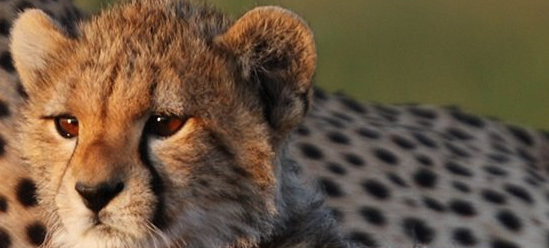
\includegraphics[width=\linewidth]{202008.png}

\vspace{-155pt}
\hfill
\begin{minipage}{7.1cm}
\begin{tcolorbox}[opacityframe=0, opacityback=0.6,width=7cm,sharpish corners]
{ { \heiti \color{symbolcol}“}我有一双水汪汪的眼睛,两只又短又尖的耳朵,身上穿着一条又黄又美的裙子,上面还布满了黑点,舒服极了。我有四只长长的腿,要是我的伙伴们跟我比跑步,还远远跑不过我呢!我还有一条长长的尾巴,像一条绳子,总是一甩一甩的。{\heiti \color{symbolcol}”}}
\end{tcolorbox}
\end{minipage}	


\vspace{13pt}

\cvsection{教育背景}

\cvsbsection{2007.6-2009.9}{硕士学位 \quad 电子工程 }{清华大学}
\cvdetail{毕业论文:\kaishu 基于xxx对xxx的研究}

\cvdetail{主修课程: 数学分析,常微分方程,微分方程定性理论,高等代数,概率论与数理统计,近代概率论,实变函数与泛函分析,计算方法,算法分析等}

\cvdetail{blahblah}

\cvsbsection{2007.6-2009.9}{学士学位  \quad 信息科学 }{清华大学}

\cvdetail{主修课程: 数学分析,常微分方程,微分方程定性理论,高等代数,概率论与数理统计,计算方法,算法分析等}

\cvdetail{毕业论文:\kaishu 基于xxx对xxx的研究}

\cvdetail{blahblah}



\cvsection{工作经历}

\cvsbsection{2007.6-2009.9}{扫厕所}{中国石油化工集团公司}
\cvdetail{毕业论文:\kaishu 基于xxx对xxx的研究}

\cvdetail{blahblah}

\cvdetail{blahblah}

\cvsbsection{2007.6-2009.9}{刷盘子}{荷兰皇家壳牌石油公司}

\cvdetail{毕业论文:\kaishu 基于xxx对xxx的研究}

\cvdetail{blahblah}

\cvdetail{blahblah}

\cvsection{获奖\& 证书}
\cvprizedetail{2017.6}{“高教社杯”数学建模竞赛}{全国一等奖}

\cvprizedetail{2017.6}{“高教社杯”数学建模竞赛}{全国一等奖}

\cvprizedetail{2017.6}{“高教社杯”数学建模竞赛}{全国一等奖}


\cvprizedetail{2017.6}{“高教社杯”数学建模竞赛}{全国一等奖}

\cvprizedetail{2017.6}{“高教社杯”数学建模竞赛}{全国一等奖}

\cvprizedetail{2017.6}{“高教社杯”数学建模竞赛}{全国一等奖}

\end{rightcolumn}









%---------------------------------
%            左边栏
%---------------------------------
\begin{leftcolumn}
\vspace*{-0.9em}

\leftsection{个人信息}{
\begin{tabular}{rl}
出生日期:&1994.9\\
名族:&汉\\
政治面貌:&团员\\
身高:&180cm\\
体重:&70kg
\end{tabular}
}

\leftsection{联系方式}{
\information{\faEnvelope}{example@gmail.com}\\
\information{\faTwitter}{@example.com}\\
\information{\faMapMarker}{山西省西山县高老庄}\\
\information{\faGlobe}{\url{http://example.example.org/}}\\
\information{\faLinkedin}{\url{ http://www.linkedin.com/in}}\\
\information{ \faPhone}{15511008888}
}

\leftsection{编程技能}{  
\begin{tabular}{rl}
JAVA & \textcolor{symbolcol}{\faStar \faStar \faStar \faStarHalfEmpty \faStarO}\\
R  &  \textcolor{symbolcol}{\faStar \faStar \faStarHalfEmpty \faStarO \faStarO}\\
python  &  \textcolor{symbolcol}{\faStar  \faStarHalfEmpty \faStarO \faStarO \faStarO}\\
MATLAB  &  \textcolor{symbolcol}{\faStar  \faStarHalfEmpty \faStarO \faStarO \faStarO}
\end{tabular}
}
\leftsection{研究领域}{
机器学习\\
深度学习\\
数据分析\\
数据挖掘
}

\leftsection{兴趣爱好}{
读书\\
\LaTeX{} 排版\\
乒乓球\\
听音乐
}

\leftsection{英语能力}{
通过CET-6,较好的读写能力
}



\end{leftcolumn}
\end{paracol}

\end{document}
